\documentclass{article}
\usepackage[utf8]{inputenc}
\usepackage[spanish]{babel}
\usepackage{listings}
\usepackage{graphicx}
\graphicspath{ {images/} }
\usepackage{cite}

\renewcommand{\familydefault}{\sfdefault}

\begin{document}

\begin{titlepage}
    \begin{center}
        \vspace*{1cm}
            
        \Huge
        \textbf{IMPLEMENTACION PARCIAL-2}
            
        \vspace{0.5cm}
        \LARGE
        
            
        \vspace{5cm}
            
        \textbf{Esteban Felipe Güiza Piñeros}\\
        \textbf{Jose Manuel Rivera Villa }
            
        \vfill
            
        \vspace{0.8cm}
            
        \Large
        Despartamento de Ingeniería Electrónica y Telecomunicaciones\\
        Universidad de Antioquia\\
        Medellín\\
        Septiembre de 2021
            
    \end{center}
\end{titlepage}

\tableofcontents
\vspace{15cm}


\begin{center}
\Huge
\section{CLASES IMPLEMENTADAS: }
\end{center}

\vspace{1cm}

En esta seccion se presentara las clases implementadas para este proyecto, describiendo brevemente  el proceso de desarrollo, y su funcionamineto dentro del sistema.

\subsection{Imagen}
Esta diseñada con atributos de otros clases y metodos para la estructura  de la matriz, para  el redimensionamiento de la imagne que ingrese el usuario, y asi posteriormente modificarla. 
\subsection{QObject}
Metodos internos de desplazamiento y estructuracion, contiene componentes para desarrollo de interfaces gráficas de usuario.

\subsection{QImage}
 Proporciona una representación de imagen independiente del hardware que permite el acceso directo a los datos de píxeles y se puede utilizar como dispositivo de pintura para modificarla o obtener informacion de sus pixeles.

\subsection{QVector}
Es necesario para  el uso de estructuras de datos,y el almacenamiento de los valores.


\subsection{QColor}
Esta clase prporciona colores basados en valores RGB, que se pueden ser creados con valores espaceificos o extraidos de otros formatos.

\subsection{QString}
Esta clase nos permite crear cadenas para manipular la informacion y ademas convertirlas en otros tipos de datos.

\subsection{math.h}
Esta clase proporciona varias funciones matematicas, que nos fueron utiles para crear un margen de error, en el proceso de redimensionalizacion y evitar posibles errores en los valores de los colores del RGB.


\vspace{10cm}

\begin{center}
\Huge
\section{ESQUEMA DE CLASES: }
\end{center}
\subsection{Desarrollo:}
La proceso inicial del proyecto se inicio con la clase Image que se desarrollo con atributos  privados de clases como -QImage-,-QColor- y -QVector-, estas contenian elementos necesarios para el redimencionamiento y manipulacion de la imagen  y  tambien publicos con el uso de clases y metodos necesesarios como -QString-,-QVector-, y el uso MatColor que fue un atributo que nos permitia guardar una imagen en un formato RGB con   matrices de diferentes dimensiones.

\subsection{Estructura:}
La estructara se creo a partir del cambio de resolucion de la imagen o a lo que se le define como sobremuestreo o submuestreo, con un condicional que verificara el tamañano de la imagen y nos dira que funcion debemos aplicar para incorporar ese cambio en una matriz de 10x10, que fue establecida en el ciruito de Tinkercad.Para eso, se separa la imagen en segmentos establecidos con las medidas de alto y ancho, y se crea una matriz con los valores de sus colores, despues se  redimenciona esa matriz y  se tomo el promedio de los clores primarios del RGB, y posteriormete se establecio un margen de error para que los valores se aseguraran en un rango obtimo. 


\vspace{1cm}

\begin{figure}[h]
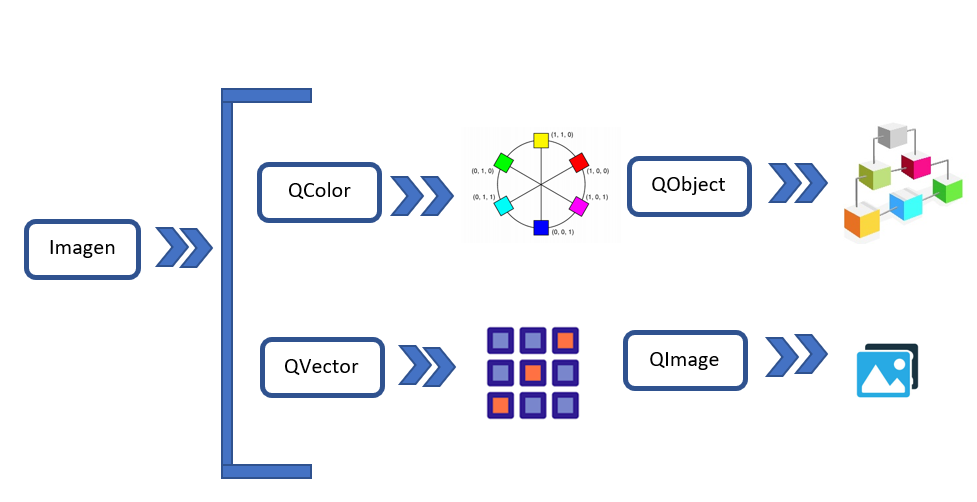
\includegraphics[width=12cm]{estructura.PNG}
\centering
\caption{}
\label{fig:tipos}
\end{figure}


\vspace{10cm}
\begin{center}
\Huge
\section{MODULOS DEL CODIGO: }
\end{center}

\subsection{Definiciones:}
El funcionamiento de las clases y los metodos que se utilizaron desde la ejecucion del codigo, comienza desde la utlizacion de la clase QImage, para la lectura de la imagen suministrada por el usuario.
Posteriormente se realiza la creacion de la clase Imagen, que cuenta con atributos de otras clases para su funcionamiento y tambien cuentan con metodos publicos tales como:

\begin{figure}[h]
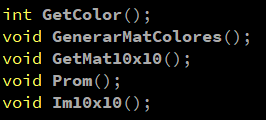
\includegraphics[width=9cm]{image.png}
\centering
\caption{}
\label{fig:tipos}
\end{figure}

En el orden de la ejecucion de los metodos, inicilamente se encargan de suministrar los datos de los colores representados por el RGB de la imagen, despues asignamos las dimensiones de la matriz con esos colores, y se asignamos  las secciones donde sacaremos el promedio de cada uno de las secciones y redimenecionaremos de esos espacios para poder utilizar los elementos en matriz de 10x10.



\subsection{Visualizacion:}
La salida del programa será un archivo txt que contendrá el segmento de código que debe ser agregado en el controlador de la matriz de LEDs de la plataforma de Tinkercad.El esquema de estos datos sera un conjunto de tres valores, segun el formato del RGB, que cuenta con circuito lógico integrado.


\begin{figure}[h]
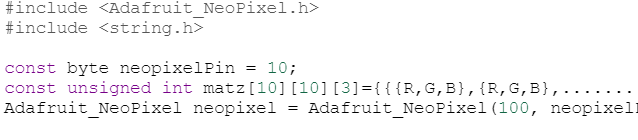
\includegraphics[width=12cm]{arduino.PNG}
\centering
\caption{}
\label{fig:tipos}
\end{figure}





\vspace{1cm}
\begin{center}
\Huge
\section{ESTRUCTURA DEL CIRCUITO: }
\end{center}
El circuito integrado de cada LED  almacena 3 bytes, un byte para cada color, que esta dimensionado en un matriz [10][10][3] con un arreglo de LED Neopixel, donde se icorporara los numeros suministrados por el codigo, que representaran los bytes.

\begin{figure}[h]
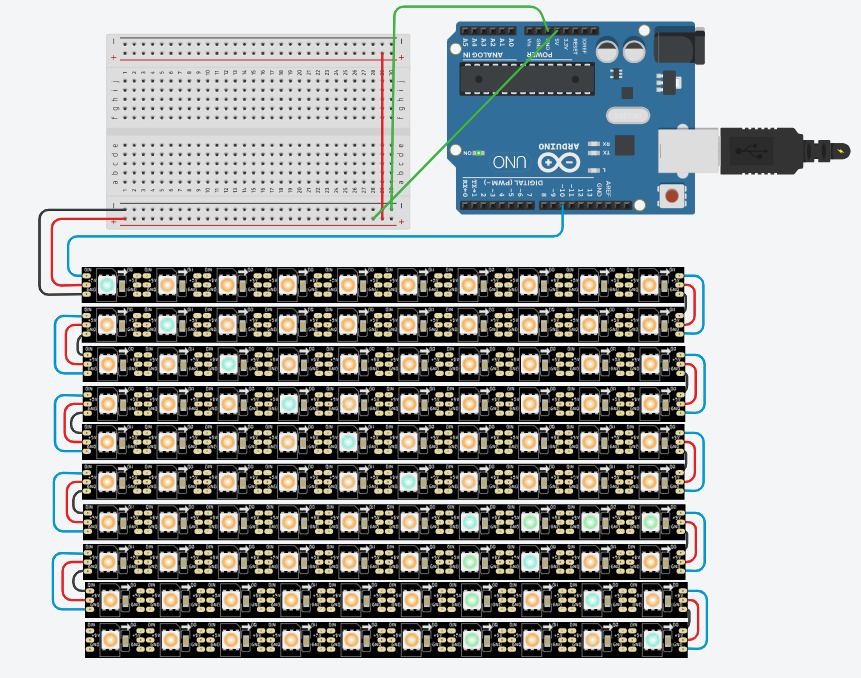
\includegraphics[width=12cm]{estruc.PNG}
\centering
\caption{}
\label{fig:tipos}
\end{figure}

\begin{figure}[h]

\includegraphics[width=3cm]{prueba.png}
\centering
\caption{}
\label{fig:tipos}
\end{figure}



\vspace{2cm}
\begin{center}
\Huge
\section{PROBLEMAS PRESENTADOS: }
\end{center}

•Uno de los problemas iniciales fue el planteamiento de como redimencionar la imagen, ya que los valores que obtenimos no eran acordes a las dimenciones  planeadas para la amatriz en Tinkercad, utilizamos vectores para el almacenamiento de  los datos cuando logramos crear la secciones para promediar el color de los pixeles.

 \vspace{1cm}
 
•Para el proceso de Submuestreo calculamos por secciones los colores del RGB y sacamos un promedio acorde a las espacificaciones de la matriz, pero algunos de los datos no mostraban el color que teniamos determinado, ya que los valores excedian el rango del promedio, por la tanto creamos un condicional que restringia los valores que sobrepasaran el promedio y calculamos un margen de error. 

 \vspace{1cm}
 
•Para el redimencionamiento en el sobremuestreo se presentaron algunos problemas para establecer el agrandamiento de la imagen, como cual seria  el valor aproximado que necesitamos para ampliar las secciones de la imagen  o como manejabamos los espacios vacios que se añadian al cambiar el tamaño de la imagen.


 \vspace{1cm}


 \vspace{8cm}
\begin{center}
\Huge
\section{MANUAL DE USO: }
\end{center}
\subsection{Entrada:}
•Es necesario que el usuario ya tenga un archivo de la imagen  que desea representar, sin importar su formato de imagen.

•La imagen debe ser guardada en una carpeta especifica llamada " Imagenes"

•Al Iniciar la aplicacion la terminal de Qt le pedira  el nombre de archivo  que desea representar para incorporarlo a la ruta.

•Ejemplo de ruta:
\vspace{0.3cm}

       "../Parcial-2/imagenes/imagen.jpg"
\vspace{0.3cm}

•Bebe escribir el nombre exacto del archivo y epecificar su tipo de formato:

\vspace{0.3cm}
          NOMBRE.(tipo de formato)

\subsection{Datos Suministrados:}

•La aplicacion procesara la imagen de acuerdo a sus dimensiones y entregara un conjunto de datos para respresntarla.
\vspace{0.2cm}

•Ejemplo del Conjunto de Datos:
\vspace{0.5cm}

[10][10][3]=((254,158,2),(231,143,4),(158,101,12),(128,115,97),.......)


\subsection{Ingreso de los Datos:}

•Se debe ingresar manualmente los datos suministrados por la apalicacion en la posicion del arreglo que ya fue establecido para la matriz 10x10.

•Los datos deben ir despues de la definicion de arreglo:

\vspace{0.2cm}
    matz[10][10][3]=

\vspace{0.2cm}
•Segmento donde deben ir los valores:

\begin{figure}[h]
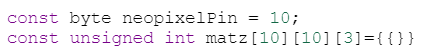
\includegraphics[width=12cm]{det.PNG}
\centering
\caption{}
\label{fig:tipos}
\end{figure}

\end{document}


